\documentclass[conference,compsoc]{IEEEtran}
\usepackage{amssymb,amsmath,amsthm}
\usepackage{algorithm}
\usepackage{algpseudocode}
\usepackage{graphicx}
\usepackage{caption}
\usepackage{cite}
\usepackage{sidecap}
\usepackage{lipsum}

\newtheorem{theorem}{Theorem}
\newtheorem{definition}{Definition}

\begin{document}

\title{A Branch-and-Cut Algorithm for Constrained Graph Clustering}

\author{\IEEEauthorblockN{Behrouz Babaki}
\IEEEauthorblockA{Dept. Computer Science\\
KU Leuven, Belgium}
\and
\IEEEauthorblockN{Dries Van Daele}
\IEEEauthorblockA{Dept. Computer Science\\
KU Leuven, Belgium}
\and
\IEEEauthorblockN{Tias Guns}
\IEEEauthorblockA{Dept. Business, Technology, \\and Operations\\
VUB, Belgium}}

\maketitle

\begin{abstract}
Representing the relationships among instances as a graph is a common practice in bio-informatics. These relationships should be taken into account in the data analysis. Including these relationships in a clustering task amounts to a graph partitioning problem. In this paper, we introduce a new graph partitioning problem with applications in analysis of biological networks. We present two mixed integer programming formulations for this problem. We also present a branch-and-price algorithm to deal with the exponential number of constraints. The experiments suggest that this approach scales to the real-world instances.
\end{abstract}

\section{Introduction}
\label{introduction}

Clustering is the task of partitioning a set of instances into
homogeneous subsets. Most clustering algorithms only take the features
of individual instances as input. However, it is also possible to
encode the relationships between instances as a graph and include this
information in the clustering task. When the instances form the nodes
of a graph, the clustering task is also called \emph{graph
  partitioning}. Given the abundance of relational data in social
network analysis and bioinformatics, it is not a surprise to see
numerous applications of graph partitioning in these fields. However,
graph partitioning has also applications in route planning, image
processing, VLSI design, and parallel processing~\cite{Survey}.

Motivated by an application in the analysis of biological networks, we
introduce the following graph partitioning problem: Given a Graph
$G=(V, E)$ and a positive integer $k$, partition the graph into $k$
connected components. We also assume that there are a set of penalties
for co-membership of certain pairs of nodes in the same cluster. We
desire two properties for the output partitioning: First, we want to
avoid obtaining components that are too small. Second, the total
weight of penalties should be as small as possible.

We formulate this problem as mixed integer programming (MIP)
problem. Recently, there has been an interest in such
approaches from the \emph{declarative data mining}
perspective~\cite{vran,me}. This perspective encourages formulating
data mining problems as models in constraint satisfaction/optimization
frameworks (e.g. constraint programming and integer programming). One
of the motivations for doing so is that existing algorithms can be
extended to new problems by modification of addition of constraints.

We have two contributions in this paper:
\begin{itemize}
\item We identify a new graph partitioning problem with applications in analysis of biological networks, and present a MIP formulation for solving it. 
\item We present a branch-and-price algorithm to improve the performance and scalability of our method. 
\end{itemize}

The rest of this paper is structured as follows:  In
section~\ref{sec:motivation} we present the application that motivates
this problem.  In section~\ref{sec:definition} we introduce the formal
definition of the problem and present the sketch of a MIP formulation.
In section~\ref{sec:connectivity} we introduce two formulations for
the connectivity constraints. Both these formulation involve an
exponential number of constraints. We then present a method for
including only a sufficient subset of these constraints to the
model. Section~\ref{sec:experiments} contains some experiments and
discussions. We review the related literature in section~\ref{sec:related}, and conclude the paper in section~\ref{sec:conclusion} with conclusions and suggestions for future work.


\section{Motivating application}
\label{sec:motivation}

Cancer sequencing has become fairly commonplace, enabling the genome-wide measurement of somatic mutations across large groups of cancer patients.
The key challenges when interpreting these data are to detect the genes that affect the creation and development of cancer and to gain an understanding of how they interact with one another.

Initially, the main was focus was placed on solely detecting the key driver mutations. More recently \cite{}, methods have been development that aim to exploit the information contained in the human interaction network. By incorporating such biological pathway information, a superior selection and understanding of genes and their interactions becomes possible. These new methods do introduce new challenges. While the extracted genes and interactions may prove statistically relevant across a large set of patients, the underlying mechanisms that affect individual patients can not always be easily distinguished, as these pathways might connect to one another or potentially overlap.

However, it is known that the creation and growth of tumors follows a clonal evolutionary model. For a tumor this means that following the disruption of a single gene, a fitness increase is no longer received when disrupting additional genes in the triggered pathway. As such, multiple mutations within a single pathway are often redundant, and consequently less commonly observed on the level of individual patients. This property can be exploited to distinguish pathways from one another.


Consider a sub-graph of the human interaction network containing only those genes and interactions that were identified as being highly relevant to a particular cancer. Each node represents a gene or gene product, and each edge represent an interaction between a pair of nodes. The graph may consist of multiple connected components. It is our goal to separate distinct pathways from each of these components. Each pathway is connected, thus motivating the usage of connectivity constraints. The rule that pairs of mutated genes within individual patients should not be assigned to the same pathway can be imposed using can-not-link constraints. Since there are several known exceptions to this rule, we require the usage of soft constraints. The penalty associated with violating such a constraint is a function of the harm associated with the mutations and the number of patients in which that pair was observed.

%This evolutionary property can be exploited to understand cancer mechanisms and identify driver mutations by searching for groups of genes that display mutual exclusivity with each other (i.e. groups of genes which have mostly one mutation per tumor).
%A first series of methods that analyze gene sets assume that, because of the clonal properties of cancer cells, recurrent mutations should occur at the pathway level rather than at single gene level. These methods search for



\section{Problem definition}
\label{sec:definition}

We assume that the reader is familiar with basic graph theory. Here we quickly review some important basic notions: A graph $G=(V, E)$ consists of a set of nodes $G$ and a set of edges $E$. A graph is \emph{simple} if it does not have any loops or double edges. A graph is \emph{connected} if there is a path between each pair of its nodes. The nodes on a path except the first and last ones are called the \emph{intermediate nodes}. A \emph{simple path} is a path with no cycles. The induced subgraph of $G$ on a set of nodes $W$ has $W$ as its node-set and contains those edges in $G$ which have both endpoints in $W$. 

Consider a simple undirected graph $G=(V, E)$. Our goal is to partition $V$
into $k$ subsets (called \emph{clusters} from now on), such that the
subgraph induced by each subset is connected. Our preference is to avoid
having clusters that contain only a small number of nodes. To enforce
this preference, we define one of our goals as maximizing the size of
the smallest cluster. Moreover, there exists a set of tuples
$C = \{(u, v, w): u, v \in V, w \in \mathbb{R}^+\}$ which indicates that
including $u$ and $v$ in the same cluster will induce a penalty of $w$. We denote all edges $(u, v)$ such that $(u, v, w) \in C$ by $E_C$. Our second goal is to minimize the sum of such penalties.

To include both goals in the objective function, assume that $S$ is the
size of the smallest cluster and $W$ is the total penalty. We define the
objective function as maximizing $S + \gamma W$ where $\gamma$ is a
parameter specified by user which determines the relative importance of
each of the two goals.

We can formulate this problem as an integer linear program. The main
decision variables in this formulation are those that determine the
assignment of vertices to the clusters. In our formulation, the binary
variable $x_{ij}$ indicates whether or not vertex $i$ is included in
cluster $j$. We know that each vertex is assigned to exactly one
cluster. This can be enforced by the following set of constraints:

\begin{equation}
\sum_{j=1}^k x_{ij} = 1 \quad \forall i \in \{1, \ldots, |V|\} \label{cons:assign}\\
\end{equation}

To include the penalties in the model, we introduce additional
variables. The binary variable $y_{uvj}$ is equal to one if and only if
vertices $u$ and $v$ are both included in the $j$th cluster. To enforce
this property, we add the following constraints to the model:

\begin{equation}
y_{uvj} \geq x_{uj} + x_{vj} -1 \quad \forall j \in \{1, \ldots, k\}, \forall (u, v) \in E_{C}
\end{equation}

If both $x_{uj}$ and $x_{vj}$ are equal to one, this constraint forces
$y_{uvj}$ to be equal to one. Otherwise, $y_{uvj}$ can be either zero or
one. However, as we will see, $y_{uvj}$ is included in the objective
function with a negative coefficient. Hence the optimization procedure
will automatically fix $y_{uvj}$ to zero in such cases.

Finally, we introduce an integer variable $s$ which represents the size
of the smallest cluster. The domain of $s$ is
$\{0, \ldots, \lceil \frac{|V|}{k} \rceil \}$. The following constraints
ensure that $s$ represents the size of the smallest cluster:

\begin{align}
s \leq \sum_{i=1}^{|V|} x_{ij} \quad \forall j \in \{1, \ldots, k\}
\end{align}

Our formulation so far does not ensure that the nodes in each cluster
are connected. For now assume that constraint
$\mathsf{connected}(x_{1j}, \ldots, x_{|V|j})$ enforces the connectivity of
cluster $j$. We will discuss the exact formulation of this constraint in
the next section. 

The model that we defined in this section is presented
below:

\begin{align}
& \text{maximize} \quad s + \gamma \sum_{j=1}^{k} \sum_{(w, u, v) \in C} w  y_{uvj}  \\
&\textit{s.t.}                                                                       \nonumber \\
&\sum_{j=1}^k x_{ij} = 1                                                             \forall i \in \{1, \ldots, |V|\} \\
& y_{uvj} \geq x_{uj} + x_{vj} -1                                                    \forall j \in \{1, \ldots, k\}, \forall (u, v) \in E_{C} \\
& s \leq \sum_{i=1}^{|V|} x_{ij}                                                     \forall j \in \{1, \ldots, k\} \\
& \mathsf{connected}(x_{1j}, \ldots, x_{|V|j})                                       \forall j \in \{1, \ldots, k\} \\
& x_{ij} \in \{0, 1\}                                                                \forall j \in \{1, \ldots, k\}, \forall i \in \{1, \ldots, |V|\} \\
& y_{uvj} \in \{0, 1\}                                                               \forall j \in \{1, \ldots, k\}, \forall (u, v) \in E_{C} \\
& s \in \{0, \ldots, \lceil \frac{|V|}{k} \rceil \}                                  
\end{align}

\subsection{Overlapping clusters}
Sometimes we can allow a node to be included in more than one cluster. For example in our motivating application, \ldots. 

To modify our formulation to allow for overlapping clusters we need to ensure that each node is included in \emph{at least} one cluster. To apply this modification to our formulation, we only need to replace constraints~\ref{cons:assign} with the following inequalities:

\begin{equation}
\sum_{j=1}^{k} x_{ij} \geq 1 \qquad i \in \{1, \ldots, |V| \}
\end{equation}

\subsection{Breaking the symmetries}
Clustering problems often have an inherent symmetry which is due to the fact that the labels of clusters are arbitrary. This means that for each solution, there are $k!$ equivalent solutions that only differ by the cluster labels. We can strengthen our formulation by breaking these symmetries. \cite{SheraliD05a} suggests two options to reduce these symmetries: 1) Assign label one to the cluster that contains node one. 2) Assign labels to other clusters in the increasing order of their sizes. This translates to the following constraints:

\begin{align}
&x_{11} = 1 \\
&\sum_{i=1}^{|V|} x_{ij} \leq \sum_{i=1}^{|V|} x_{i,j+1} \qquad j \in \{2, \ldots, k\}
\end{align}

These constraints do not eliminate all symmetries (especially in the case of overlapping clusters) but still lead to improvements in performance in practice. 

\section{Enforcing connectivity}
\label{sec:connectivity}
In the previous section we did not give a concrete formulation for the constraint $\mathsf{connected}(x_{1j}, \ldots, x_{|V|j})$. In this section we present a method for enforcing this constraint.

\subsection{Enumerating all paths}
A cluster is connected if and only if there is a path between each pair of its nodes. Therefore a pair of non-adjacent nodes can belong to the same cluster only if there is at least one path between them such that all nodes on this path belong to that cluster. To encode this condition in terms of linear constraints, we will enumerate all simple paths that connect each pair of non-adjacent nodes. Consider a simple path between the nodes $u$ and $v$. Let $I$ denote the set of indices of nodes that lie between $u$ and $v$ on this path. Assume that binary variable $y$ indicates that all these nodes belong to cluster $j$. A standard translation of the relation $(y=1) \iff \land_{i \in I} (x_{ij}=1)$ to linear constraints gives the following inequality:

\begin{equation}
0 \leq \sum_{i \in I} x_{ij} - |I|y \leq |I|-1
\end{equation}

Let $P_{uv}$ denote the set of all simple paths between nodes $u$ and $v$. For a path $P_r \in P_{uv}$, let $I_r$ denote the set of indices of nodes that lie between $u$ and $v$ on $P_r$. We introduce binary variable $y_{rj}$ to indicate that all these nodes are assigned to cluster $j$. This relationship is enforced by the following constraints:
\begin{multline}
0 \leq \sum_{i\in I_r} x_{ij} - |I_r| y_{rj} \leq |I_r| - 1 \\
\forall j \in \{1, \ldots, k\}, \forall u, v \in V, (u, v) \notin E, \\ \forall r \in \{1, \ldots, |P_{uv}\}
\end{multline}

Finally, we can encode the connectivity condition by adding the following constraints:

\begin{multline}
x_{uj} + x_{vj} \leq \sum_{r=1}^{|P_{uv}|} y_{rj} + 1 \\
\forall u, v \in V, (u, v) \notin E, \forall j \in \{1, \ldots, k\}
\end{multline}

\subsection{A cutting-plane approach}
 The contents of this
section are a slight modification of the methods presented in~\cite{CarvajalCGVW13}. The presented formulation of connectivity constraints is mainly based on the notion of \emph{node-cut sets}, which we define next. 

\begin{definition}[Node-cut set]
Given nodes $u, v \in V$ that are not adjacent ($(u, v) \notin E$), a set of nodes $S \subseteq V \setminus \{u, v\}$ is a \emph{node-cut set} separating $u$ and $v$ (or simply a \emph{$uv$-node cut}) if all paths between $u$ and $v$ intersect $S$.
\end{definition}

A $uv$-node cut is \emph{minimal} if it is not a $uv$-node cut after removing any of its nodes. Figure~\ref{fig:cutset} depicts the idea of a node-cut. The following theorem shows that connectivity of a graph can be characterized by its node-cut sets. 

\begin{SCfigure}[1.4]
\centering
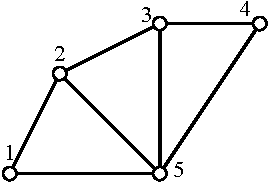
\includegraphics[scale=0.7]{images/cutset}
\caption{The sets \{2, 5\} and \{3, 5\} belong to $\Gamma(1, 4)$, but the set \{2, 3, 5\} does not.}
\label{fig:cutset}
\end{SCfigure}

\begin{theorem}
Given $U \subseteq V$ and a pair of non-adjacent nodes $u, v \in U$, there exists a path between $u$ and $v$ in the subgraph induced by $U$ if and only if all $uv$-node cuts $S$ are such that $S \cap U \neq \emptyset$.
\end{theorem}

Let us denote by $\Gamma(u, v)$ the set of all minimal $uv$-node cut sets. Then the constraint $\mathsf{connected}(x_{1j}, \ldots, x_{|V|j})$ can be formulated as follows:

\begin{multline}
\sum_{w \in S} x_{wj} \geq x_{uj} + x_{vj} - 1 \\
\forall S \in \Gamma(u, v), \forall (u, v) \in V, (u, v) \notin E
\label{eq:connectivity}
\end{multline}

This formulation adds an exponential number of inequalities to the
problem, which makes it impractical for all graphs but those with only a
few nodes. To resolve this problem, we use the \emph{cutting-plane}
method. A rough description of this method follows: We start by
including a (possibly empty) subset of these constraints and solve the
problem to optimality. The we check to see if the solution satisfies the
connectivity constraints. If it does, then this solution is also the
optimal solution for the original problem. Otherwise, we add (some of)
the violated constraints to the problem and repeat this procedure, until
all connectivity constraints are satisfied.

Note that we need a means to detect which constraints are violated by
the current solution. Since we do not want to enumerate an exponential
number of constraints, this question gives rise to another search
problem (called the \emph{separation} problem). The separation problem
is usually formulated as that of finding the \emph{most violated}
constraint.

Luckily, for the connectivity constraints, the separation problem can be
solved efficiently. Given a solution of the problem, the
separation problem for cluster $j$ can be stated as an optimization subproblem: Let us denote the value of $x_{ij}$ variables in this solution by $x^*_{ij}$. Find nodes $u$ and $v$ such that $(u, v) \notin E$ and a set $S^* \in \Gamma(u, v)$ such that the sum $\sum_{w \in S^*} x_{wj}^*$ is
minimum among all sets $S \in \Gamma(u, v)$. If $\sum_{w \in S^*} x_{wj}^* < x^*_{uj} + x^*_{vj} - 1$ then the equality~\ref{eq:connectivity}
induced by $u, v, S^*$ is violated. We solve this separation problem
once for each cluster and add the violated constraints to the problem.
If no such violated constraint is found, then the solution is optimal.

The question is now how to find $S^*$, the minimum node cut separating
$u$ and $v$. We use the following theorem to solve this problem:

\begin{theorem}
Given a graph with node capacities, the maximum flow between
two non-adjacent nodes $u$ and $v$ equals the capacity of the minimum
capacity node cut separating $u$ and $v$.
\end{theorem}

To solve the separation problem, we solve a max-flow problem for each
pair of non-adjacent nodes using values $x^*_{ij}$ as node capacities. We repeat this $k$ times, once for every cluster. This procedure is summarized in algorithm~\ref{alg:cut}.

\begin{algorithm}
\centering
\caption{The cut-generation procedure}
\label{alg:cut}
\begin{algorithmic}[1]
\State $\mathcal{C} \gets \emptyset$
\For{$j \in \{1, \ldots, k\}$}
	\For{$u, v$ such that $(u, v) \notin E$}
		\State $S^* \gets \text{min-cut}(u, v, {\mathbf{x}}^{*}_j)$ 
		\If{$\sum_{w \in S^*} x_{wj}^* < x_{uj}^* + x_{vj}^* - 1$}
			\State $\mathcal{C} \gets \mathcal{C} \cup \{\sum_{w \in S^*} x_{wj} \geq x_{uj} + x_{vj} - 1\}$ 
		\EndIf
	\EndFor
\EndFor
\State Add constraints $\mathcal{C}$ to the model
\end{algorithmic}
\end{algorithm}

Now observe that we do not need to wait for the problem to be solved to
optimality to add the violated constraints. Instead, we can do so each
time a feasible solution is found during the branch-and-bound procedure.
We can also take a step further and solve the separation problem using
the solution for the linear relaxation of the problem. We use both these
practices in our implementation.

\section{Experiments}
\label{sec:experiments}

In this section we will evaluate the suitability of our algorithms to address the motivating application. In particular, we want to answer these three questions:

\begin{description}
\item[Q1.] How does each of the two models scale in the task of overlapping clustering?
\item[Q2.] How does each of the two models scale in the task of non-overlapping clustering?
\item[Q3.] What is the effect of the $\gamma$ parameter on the trade-off between the two components of the objective function?
\end{description}


\subsection{Experiment setting}
We ran the experiments on Linux machines with 32 GB of memory. We implemented our branch-and-cut algorithm using the python interface
of \emph{Gurobi-6.5}\footnote{www.gurobi.com}. To solve the separation problem, we used the implementation of min-cut/max-flow algorithm from the \emph{NetworkX-1.11}\footnote{networkx.github.io} library. 

To use this implementation for our problem, we replaced
each undirected edge by two opposite directed edges. The capacity of
these edges is infinite. Then we replaced each vertex $v$ by two
vertices $v_{\text{in}}, v_{\text{out}}$ connected by two opposite
edges, with capacities equal to the capacity of $v$. We obtain the
minimum node cut separating $u$ and $v$ by computing the minimum cut
between $u_{\text{out}}$ and $v_{\text{in}}$ in this graph.

We followed the recipe of~\cite{CarvajalCGVW13} for adding the cuts: We added cuts to the
linear relaxation only at the root node of the branch-and-cut tree.
Moreover, when adding cuts to the relaxation, we monitored the change in
the value of objective function, and stopped adding the cuts if this
value improved less than 5\% for 10 consecutive rounds. Outside the root
node, we called the separation problem only when a feasible solution was
found.

We generated the graphs \ldots

The code and the data will be made available upon publication of this paper.

\subsection{Results and discussion}

\section{Related work}
\label{sec:related}
There are several studies that using mathematical programming
for clustering and graph partitioning
problems~\cite{Hansen}. Graph partitioning has been solved using integer programming~\cite{REF}, semidefinite programming~\cite{REF}, and quadratic programming~\cite{REF}. Techniques such as branch-and-cut~\cite{REF} and branch-and-price~\cite{REF} have been used to improve the integer programming formulations of such problems. 

The are several variants of the graph partitioning problem. When the underlying graph is a complete graph, this problem is sometimes called the \emph{clique partitioning} problem~\cite{REF}. In most variants of graph partitioning, the edges are assumed to be weighted~\cite{REF}. The number of clusters can be specified by user~\cite{REF} or decided by the algorithm. Two most prominent objective functions are 1) minimizing the total weight of the edges that have endpoints in different clusters~\cite{REF} and 2) minimizing the total weight fo the edges that have endpoints in the same cluster~\cite{REF}. Both these objectives are meant to increase the homogeneity of clusters.  

Several types of constraints are common to the graph partitioning problems. The most widely used constraint is the \emph{balance} constraint that requires the number of nodes in all clusters to be almost equal~\cite{REF}. Other types of constraints include constraint on the minimum size of a cluster~\cite{REF}, upper and lower bounds on size of clusters~\cite{REF}, and constraints on total weight of nodes in a cluster~\cite{REF}. 

The main difference of our problem with the existing problems is that the edges and nodes are not weighted. Instead, the properties of the desired clusters is specified by a set of soft \emph{can-not-link} constraints. This requires us to enforce the connectivity of clusters by means of extra constraints. The graph partitioning problem of \cite{connected} also requires such constraints. However they do not assume that the number of clusters is given, and their encoding of the clustering problem is quite different from ours. 


\section{conclusions and future work}
\label{sec:conclusion}

\bibliographystyle{IEEEtran}
\bibliography{references}

\end{document}
